\documentclass[12pt,letterpaper]{article}
\usepackage[left=1.1in,top=0.8in,right=1.1in,bottom=0.9in]{geometry}
\usepackage{amsmath,amssymb,mathtools}
\usepackage{fancyhdr}
\usepackage{booktabs}
%\usepackage{graphicx}
%\usepackage{ctex}
%\usepackage{braket}
%\usepackage{mathpazo}
%\usepackage{minted}
%\usepackage{xcolor} % to access the named colour LightGray
%\definecolor{LightGray}{gray}{0.9}
\usepackage[colorlinks=true, urlcolor=blue]{hyperref}
%\usepackage{graphicx}
%\usepackage{background}
\usepackage{setspace}
\onehalfspacing
\pagestyle{fancy}
\fancyhf{}
\lhead{ECON5253}
\rhead{Spring 2025}
%\rhead{Chang Gao}
\cfoot{\thepage}
\begin{document}
	\begin{center}
		\noindent{\Large Problem Set 6}\smallskip\\
		Chang Gao\smallskip\\
	\end{center}
	\noindent{\bf\large Q3 Data Cleaning}\medskip\\
	Here is how I cleaned the monthly housing index data scraped from China's National Bureau of Statistics. Please see the Jupyter Notebook for details.

\noindent{\bf Step 1 \& 2: Merge some split CSVs, Remove extra CSVs}\smallskip\\
	One issue with the scrapped data is that, for house of different size, for some month, the table in htmls are split. Because the table is too long, they are split into two halfs.
	
	Fortunately, the split method is consistent across time. I addressed this issue by let claude write code on: for each CSV, check if name of "specific\_city\_1" exist in the table, and if name of "specific\_city\_2" exist in the table, if not, merge.
	
	For each month, the number of csv scrapped from these htmls are around 4-12, I checked their details and found that the first few csv contains sufficient data. The format of csv and htmls differs across years. For each month I have a folder that contain these csv. I let claude worte a code that can read the first few rows (and second column since they are housing index values) of the data, and remove the csv if same data is founded. 
	
	After this step, I have 4-5 csv left in each "month" folder.
	
	\noindent{\bf Step 3: Check and keep the sufficient 4 CSVs, rename}\smallskip\\
	The sufficient 4 CSVs (xxxx\_table\_2 to xxxx\_table\_5) are: 1-new resendial housing price; 2-used resendial housing price; 3-new,small,medium,large; 4-used,small,medium,large.
	Some of the folders contains a fifth CSV (table\_1) of some summary. I did the remove of table\_1 and rename table\_2 as new table\_1, table\_3 as new table\_2...
	
		\noindent{\bf Step 4: Clear each CSV}\smallskip\\
	For each CSV, I check where its first row is variable name or the title. I removed the title and variable names.
	
	Another issue is that the data of 70 cities are put into two columns, with 35 cities in each column, I merged the separated columns.
	
	I also removed the year-to-year and month-to-month ratio from the original data set as the monthly price index have been sufficient.
	
	\noindent{\bf Step 5: Merge all the CSVs}\smallskip\\
The difficulty now comes from city names, such as "Beijing", it could be "Bei jing" or "Beijing*".
	
	\noindent{\bf Step 6: translate city names into English by dictionary}\medskip\\
\noindent{\bf\large Q4 Visualization}

\begin{figure}[htbp]
	\centering
	\begin{minipage}{\textwidth}
		\centering
		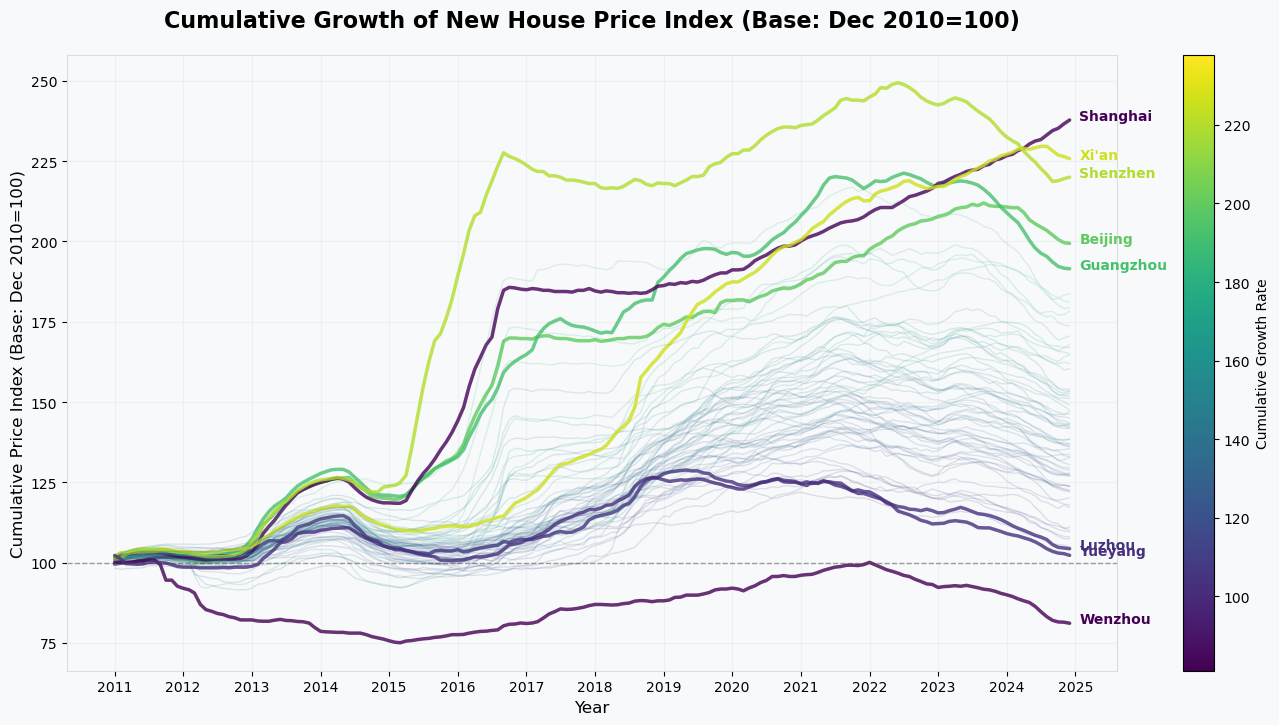
\includegraphics[width=0.7\textwidth]{PS6a_Gao.png}
		\caption{Python Output}
	\end{minipage}
	
	\vspace{0.5cm}
	
	\begin{minipage}{\textwidth}
		\centering
		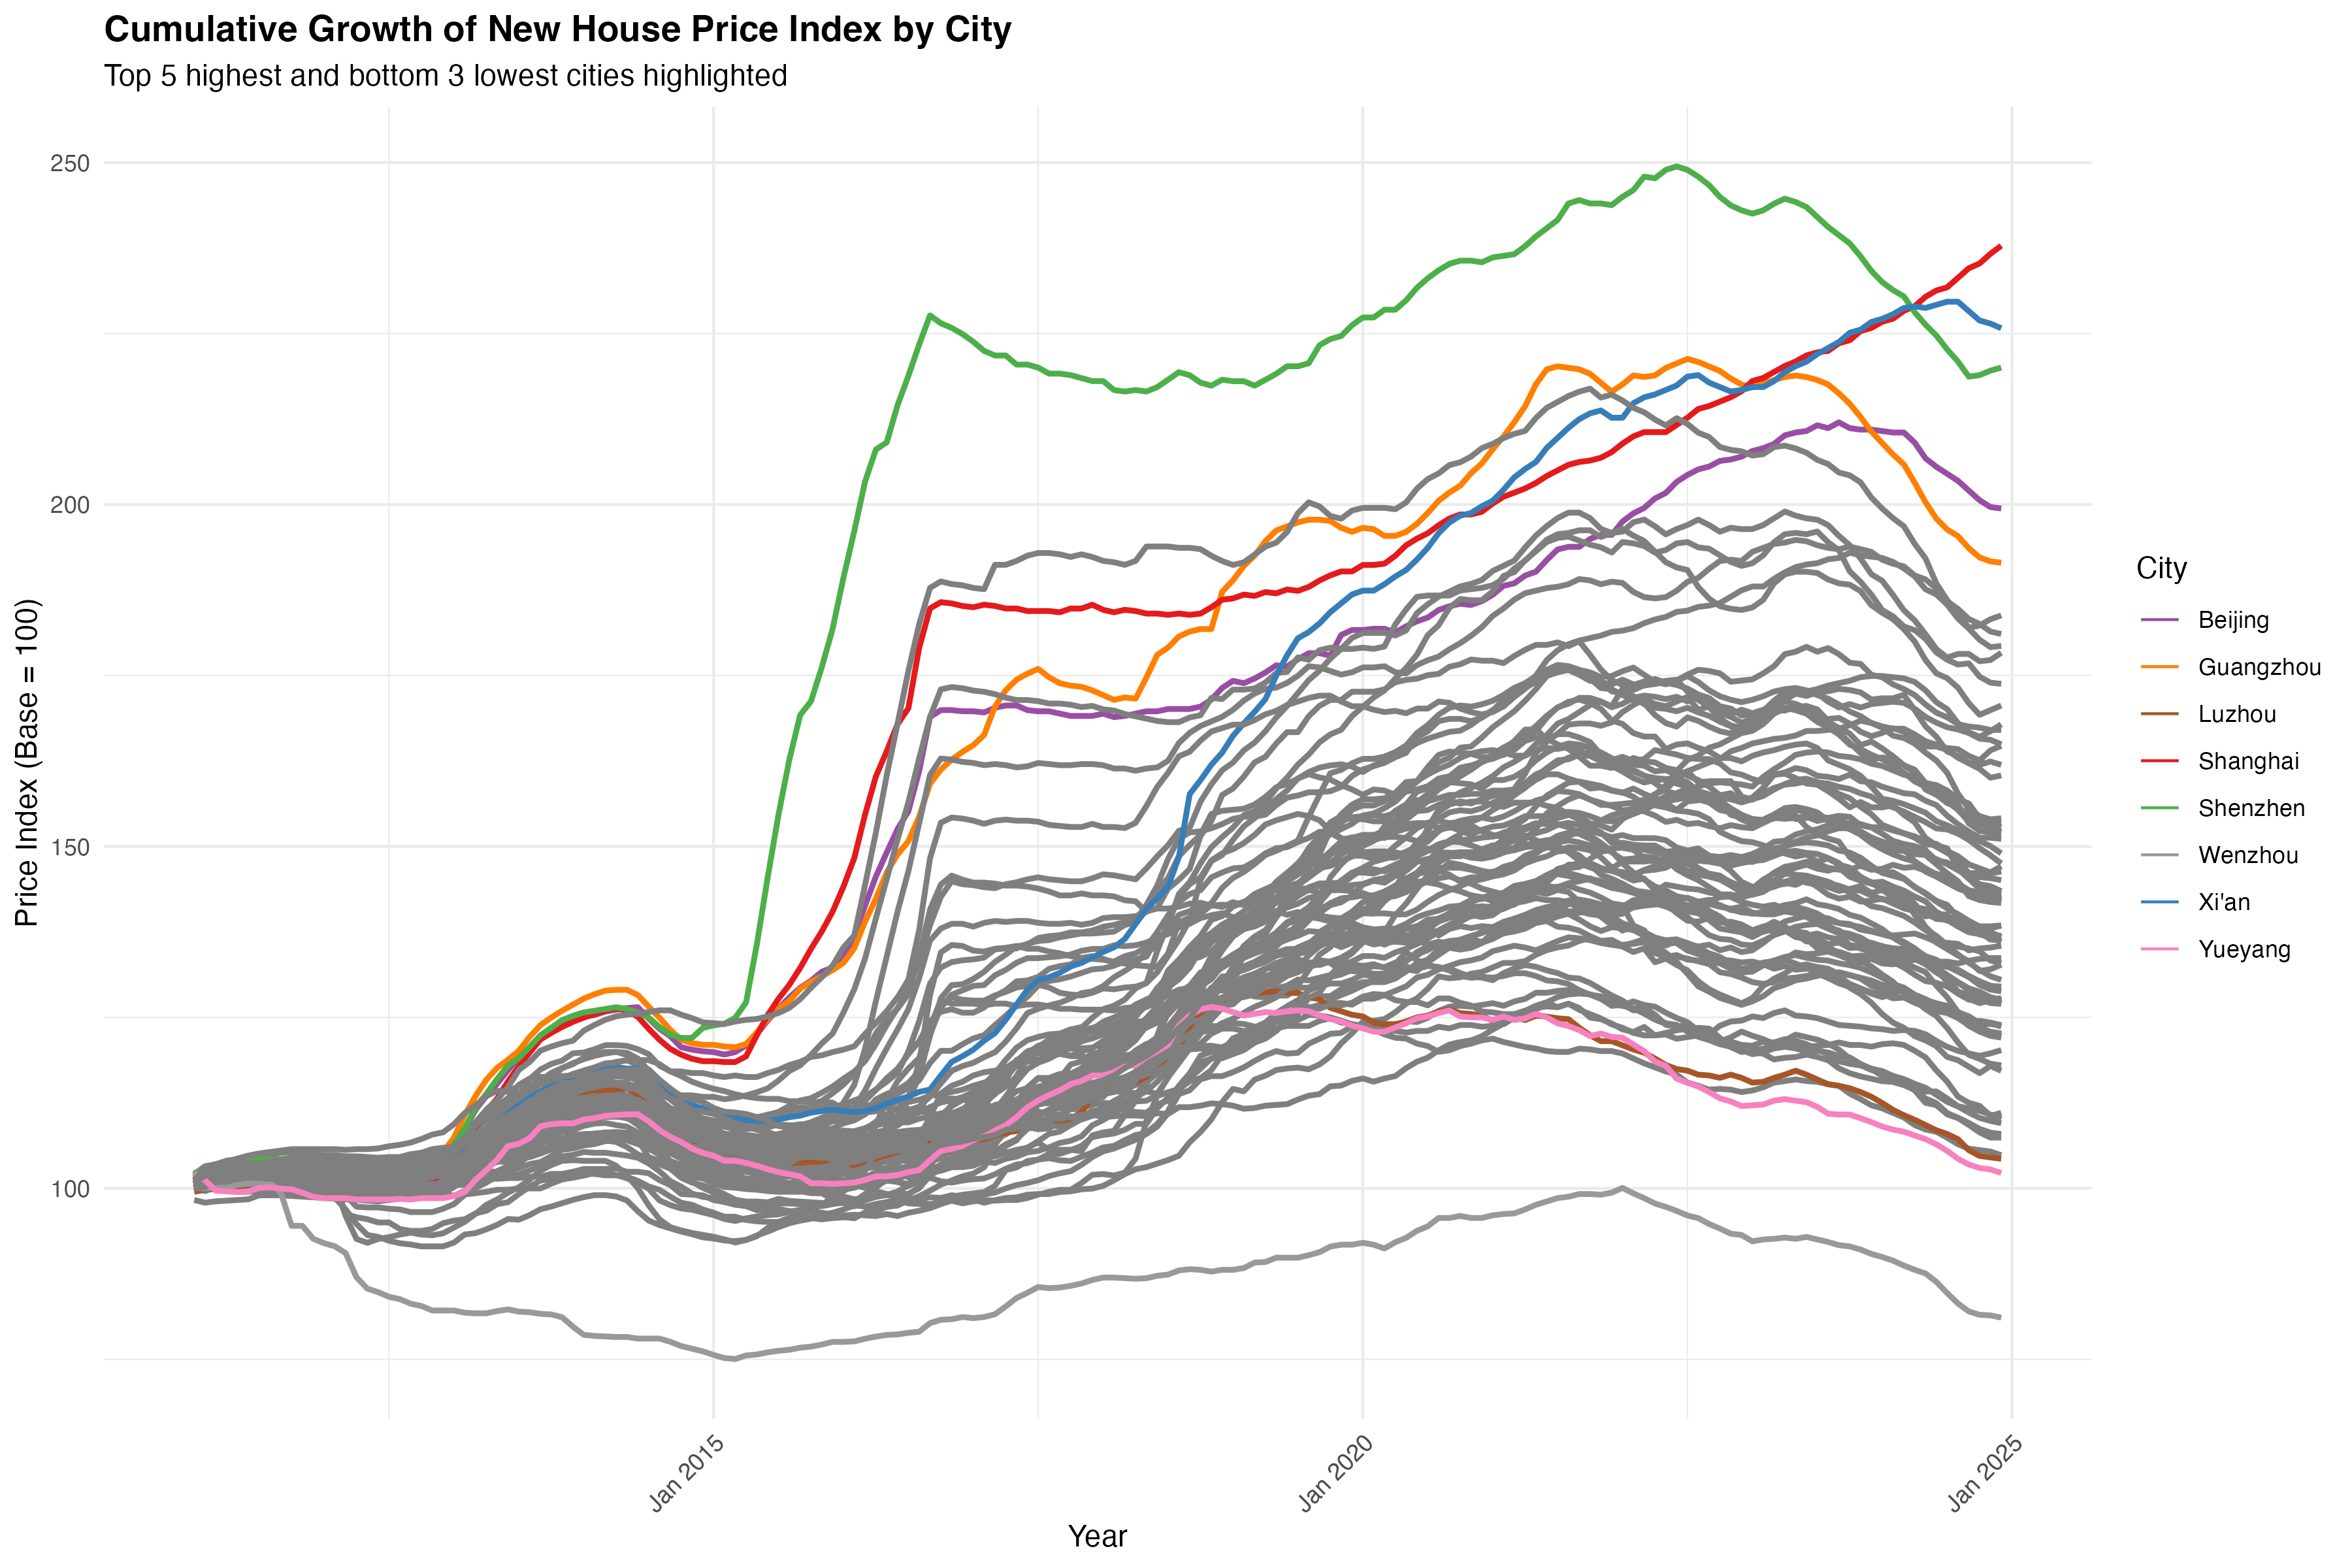
\includegraphics[width=0.7\textwidth]{PS6b_Gao.png}
		\caption{R Output}
	\end{minipage}
	
	\vspace{0.5cm}
	
	\begin{minipage}{\textwidth}
		\centering
		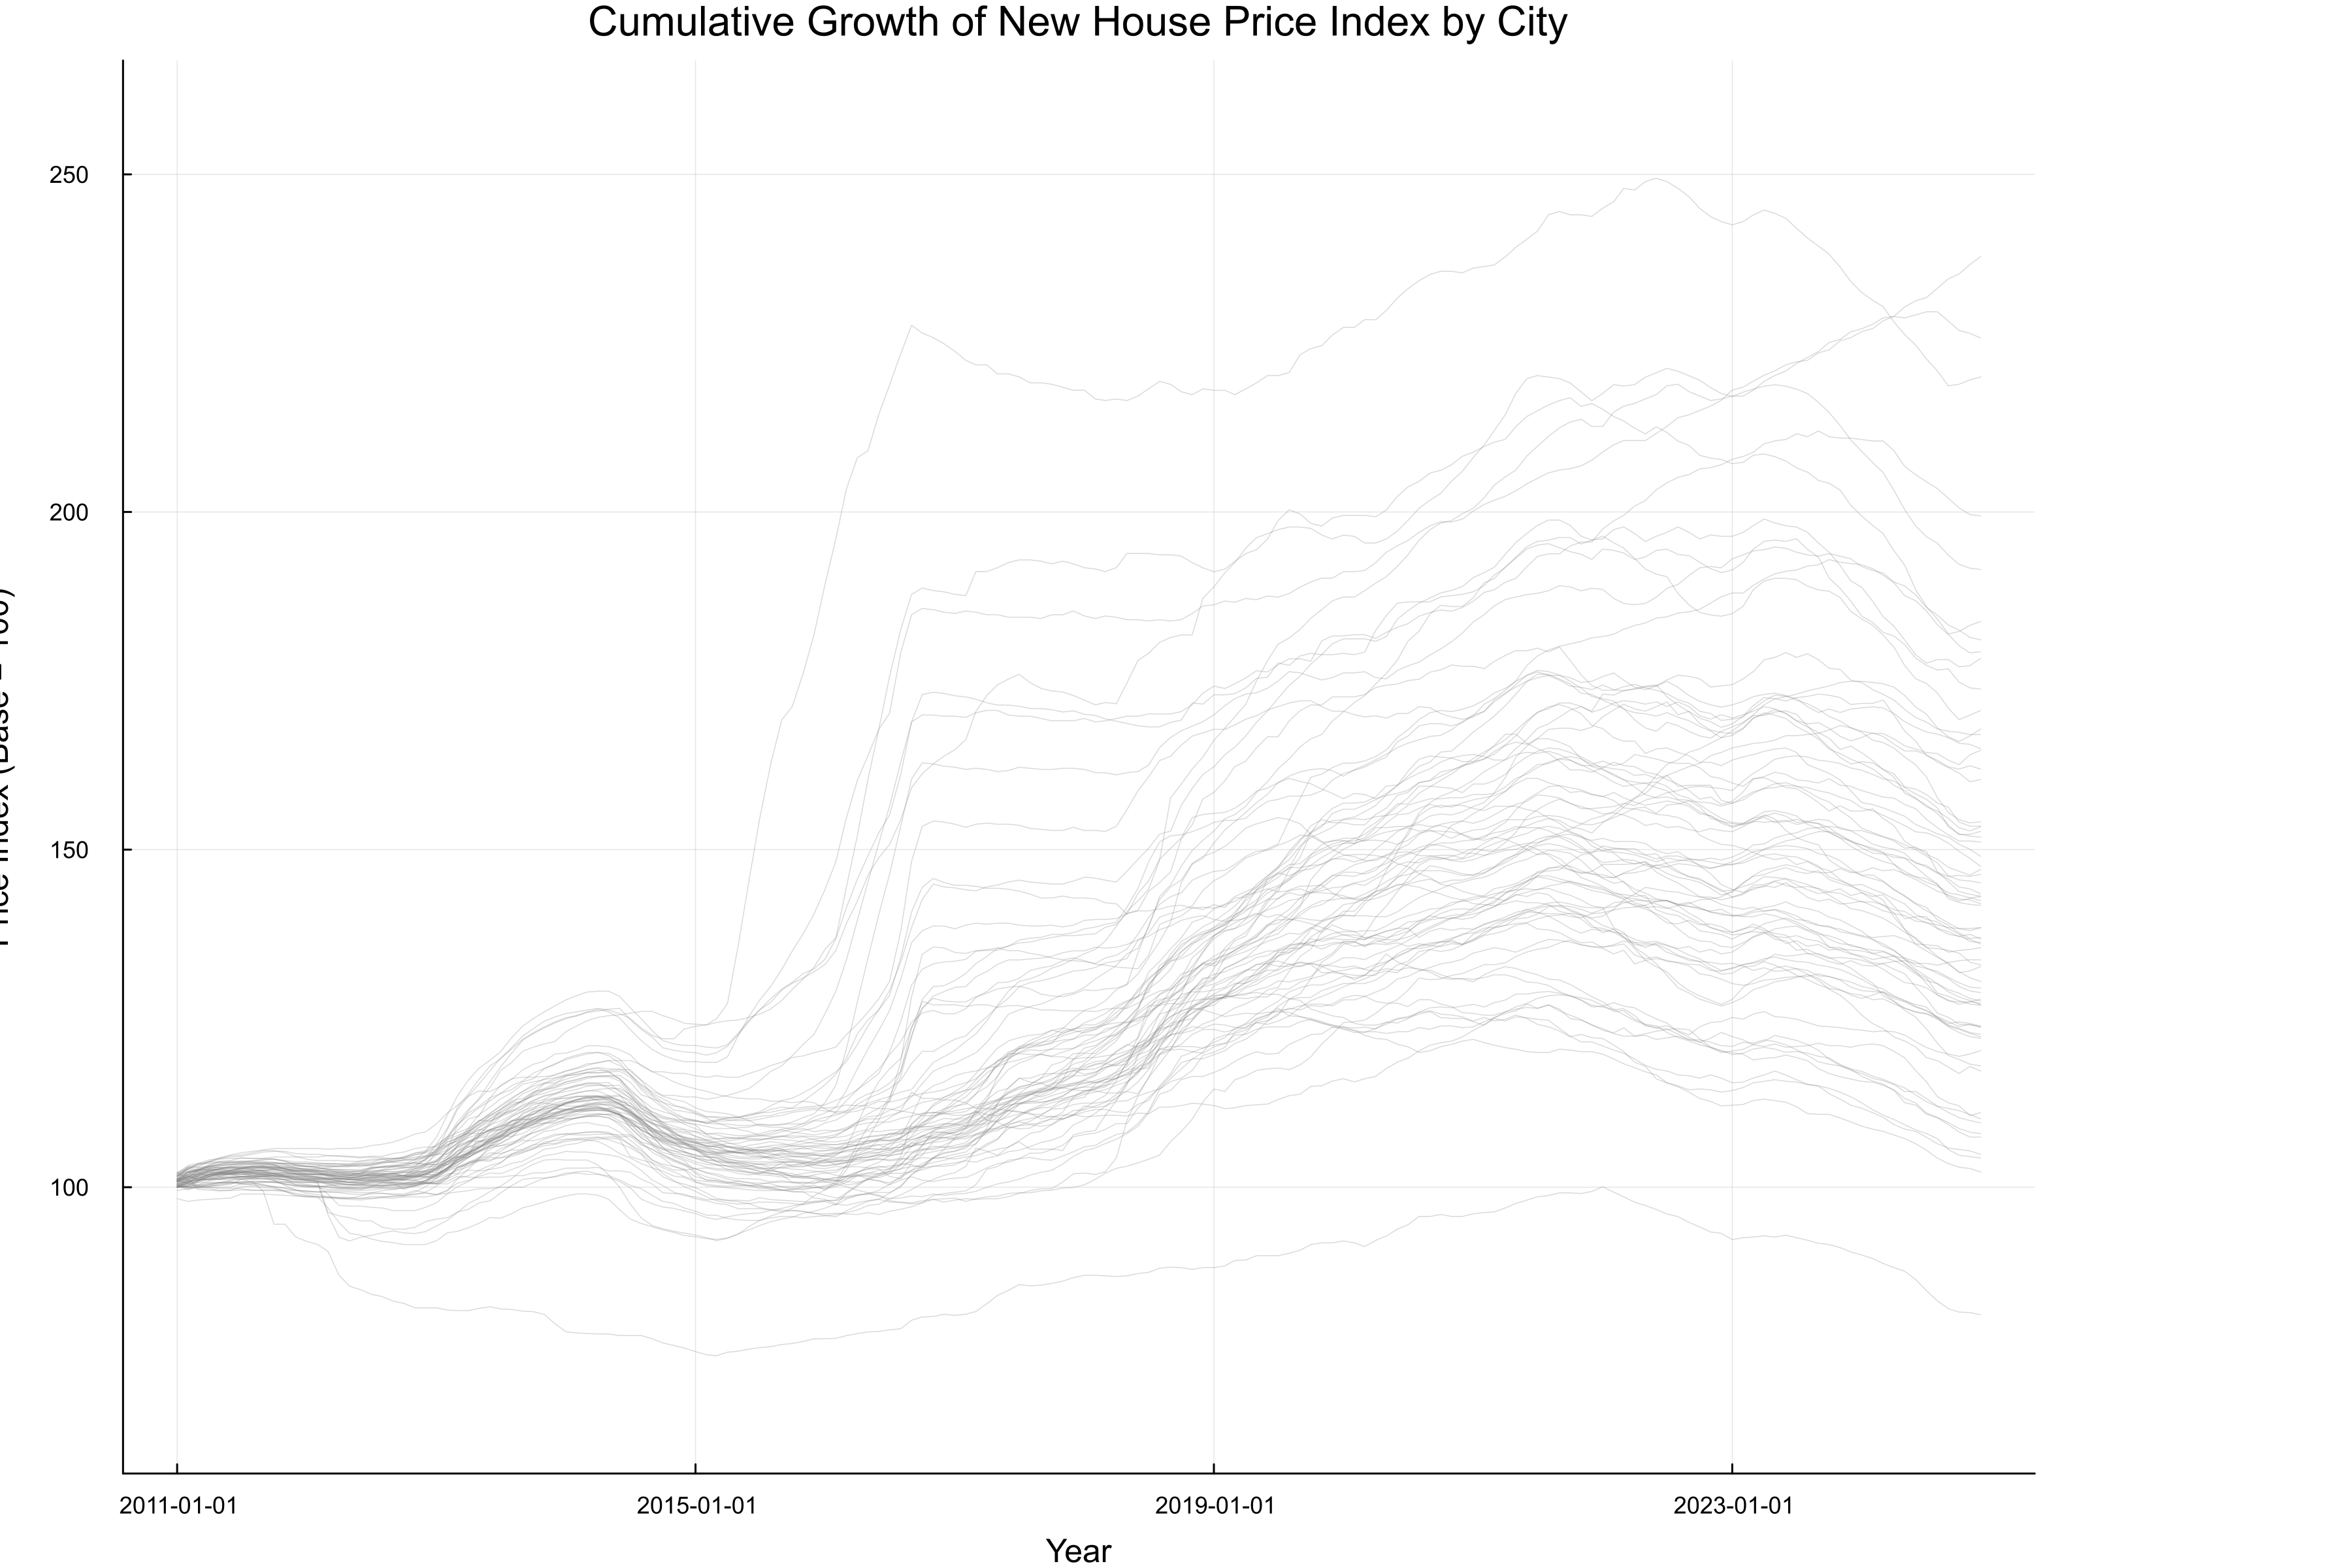
\includegraphics[width=0.7\textwidth]{PS6c_Gao.png}
		\caption{Julia Output}
	\end{minipage}

\end{figure}
	
	

	
	
	
\end{document}